\documentclass{article}

\def\ParSkip{} 
\input{../common/ryantibs}
\usepackage[normalem]{ulem}
\usepackage{centernot}

\title{Lecture 3: Linear Regression and Prediction \\ \smallskip  
\large Introduction to Time Series, Fall 2024 \\ \smallskip
Ryan Tibshirani}
\date{}

\begin{document}
\maketitle
\RaggedRight
\vspace{-50pt}

Related reading: Chapter 2 of Shumway and Stoffer (SS); Chapters 5.8, 5.10, and
7 of Hyndman and Athanasopoulos (HA).   

\section{Simple regression}

\subsection{Population version}

\begin{itemize}
\item We'll start off by learning the very basics of linear regression, assuming
  you have not seen it before. A lot of what we'll learn here is not necessarily
  specific to the time series setting, though of course (especially as the
  lecture goes on) we'll emphasize the time series angle as appropriate

\item A \emph{simple linear regression} model for a response variable $y$ and
  predictor (or covariate, or feature) variable $x$ is one in which we seek
  \emph{coefficients} (or parameters) $\beta_0$ and $\beta_1$, such that,
  informally,  
  \[
  y \approx \beta_0 + \beta_1 x
  \]
  To be clear, here $x,y$ are all real-valued (rather than multivariate) random
  variables 

\item If we had access to the full distributions of $x,y$, which is what we call
  the ``population version'' of regression, then we could ask: what is the best
  choice of parameters $\beta_0,\beta_1$ with respect to expected squared error?  

\item Mathematically, we are looking to solve
  \begin{equation}
  \label{eq:ls_pop}
  \min_{\beta_0, \beta_1} \, \E\big[ (y - \beta_0 - \beta_1 x)^2 \big]
  \end{equation}
  or in other words, we are asking for the ``line of best fit'' at the
  population level. You'll often also hear this referred to as the ``least
  squares'' problem

\item We can find the answer by differentiating the loss $Q = \E[ (y - \beta_0 -
  \beta_1 x)^2]$ in \eqref{eq:ls_pop} with respect to each parameter and
  setting it equal to zero. Differentiating inside the expectation gives:  
  \begin{gather*}
  \frac{\partial Q}{\partial \beta_0} = \E\big[ 2(\beta_0 + \beta_1 x - y) 
  \big] = 0 \\ 
   \frac{\partial Q}{\partial \beta_1} = \E\big[ 2x (\beta_0 + \beta_1 x - y)
   \big] = 0  
  \end{gather*}
 
\item As you'll show on the homework, solving this pair of equations gives the 
  \emph{population regression coefficients}:
  \begin{equation}
  \label{eq:beta_pop}
  \beta^*_1 = \frac{\Cov(x, y)}{\Var(x)}, \quad 
  \beta^*_0 = \E(y) - \beta^*_1 \E(x)
  \end{equation}

\item Recalling that \smash{$\Cor(x, y) = \Cov(x, y) / \sqrt{\Var(x) \Var(y)}$}, 
  we may rewrite the slope as 
  \[
  \beta^*_1 = \Cor(x, y) \sqrt{\frac{\Var(y)}{\Var(x)}},
  \]
  which shows that it treats $x,y$ \emph{asymmetrically}. This is important to
  remember. In general, when $y$ is the response and $x$ is the predictor, we 
  speak this relationship as the ``regression of $y$ on $x$''
\end{itemize}

\subsection{Sample version}

\begin{itemize}
\item For the ``sample version'' of linear regression, we seek $\beta_0,\beta_1$
  such that for given samples $x_i,y_i$ (covariate and response pairs), $i =
  1,\dots,n$,  
  \[
  y_i \approx \beta_0 + \beta_1 x_i, \quad i = 1,\dots,n
  \]
  but without access to the full distributions of each $x_i$ and $y_i$, just
  given these samples

\item We can imagine two ways to proceed:
  \begin{enumerate}
  \item Start from the population-level formula \eqref{eq:beta_pop}, and use 
    plug-in estimates for the covariance and variance
\item Start from the population-least least squares problem \eqref{eq:ls_pop},
  write down a sample version, then solve it
  \end{enumerate}

\item Somewhat remarkably, these two strategies end up at the same answer
  (which need not be the case)

\item For strategy 1, we use the sample covariance and sample variance, 
  \[
  \widehat{\Cov}(x,y) = \frac{1}{n} \sum_{i=1}^n (x_i - \bar{x}) (y_i -
  \bar{y}), \quad
  \widehat{\Var}(x) = \frac{1}{n} \sum_{i=1}^n (x_i - \bar{x})^2
  \]
  where \smash{$\bar{x} = \frac{1}{n} \sum_{i=1}^n x_i$} and \smash{$\bar{y} =
    \frac{1}{n} \sum_{i=1}^n y_i$} are the sample means, and plug these into
  \eqref{eq:beta_pop} to get:  
  \begin{equation}
  \label{eq:beta}
  \hbeta_1 = \frac{\sum_{i=1}^n (x_i - \bar{x}) (y_i - \bar{y})} 
  {\sum_{i=1}^n (x_i - \bar{x})^2}, \quad 
  \hbeta_0 = \bar{y} - \hbeta_1 \bar{x}
  \end{equation}
  which we call the \emph{sample regression coefficients}

\item For strategy 2, we write down the sample least squares problem   
  \begin{equation}
  \label{eq:ls}
  \min_{\beta_0, \beta_1} \, \sum_{i=1}^n (y_i - \beta_0 - \beta_1 x_i)^2 
  \end{equation}
  
\item Similar to before, denote the loss in \eqref{eq:ls_pop} by \smash{$Q =
    \sum_{i=1}^n (y_i - \beta_0 - \beta_1 x_i)^2$} and differentiate with
    respect to each parameter and set it equal to zero:
  \begin{gather*}
  \frac{\partial Q}{\partial \beta_0} =  \sum_{i=1}^n 2(\beta_0 + \beta_1 x_i -
  y_i) = 0 \\ 
   \frac{\partial Q}{\partial \beta_1} = \sum_{i=1}^n  2x_i (\beta_0 + \beta_1
   x_i - y_i) = 0  
  \end{gather*}
 
\item You'll show on the homework that solving this pair of equations leads you
  right back to \eqref{eq:beta}

\item The \verb|lm()| function in R performs linear regression. The notation you
  use is \verb|lm(y ~ x)|, where \verb|y ~ x| is called a ``formula''. This can
  be read as an instruction: ``regress $y$  on $x$''    

\item Figure \ref{fig:chicken} gives an example where we regress chicken
  prices---our response, $y$, on time---our predictor $x$. Just to give you a
  clear sense, the data are
  \begin{gather*}
  y_1 = 65.58, \, y_2 = 66.48, \, y_3 = 65.70, \dots \\
  x_1 = 2001.583, \, x_2 = 2001.667, \, x_3 = 2001.750, \dots
  \end{gather*}
  where we interpret each value of $x$ as a given year plus a fraction,
  representing the month of the year 

\begin{figure}[tb]
\centering
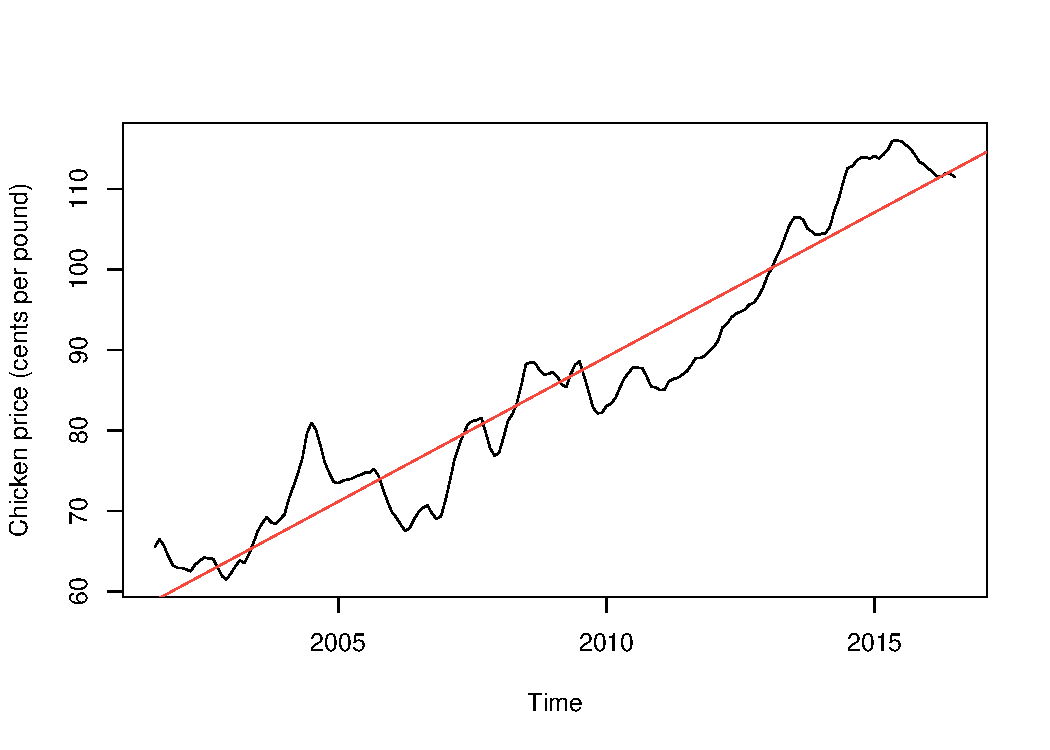
\includegraphics[width=0.875\textwidth]{fig/chicken-1.pdf}
\caption{\it Linear regression of chicken prices and on time (from SS).} 
\label{fig:chicken}
\end{figure}
  
\item After running \verb|lm()|, the resulting object is a (special) list, with
  a lot of useful  components. Calling \verb|coef()| on the object gives the
  regression coefficients   

\item Figure \ref{fig:cardio} gives another example, of a different flavor. Now
  the response $y$ is itself one time series: cardiovascular mortality in Los
  Angeles over a certain time period, and the covariate $x$ is itself another
  time series: particulate levels in Los Angeles over the same time period. The 
  top panel in Figure \ref{fig:cardio} plots them individually as time series,
  and the bottom panel plots them together, as a scatter plot, toether with the
  fitted line from linear regression. We can imagine, in a future period (beyond
  the end date of these time series), using the estimated regression
  coefficients to predict mortality from particulate levels  

\begin{figure}[p]
\centering
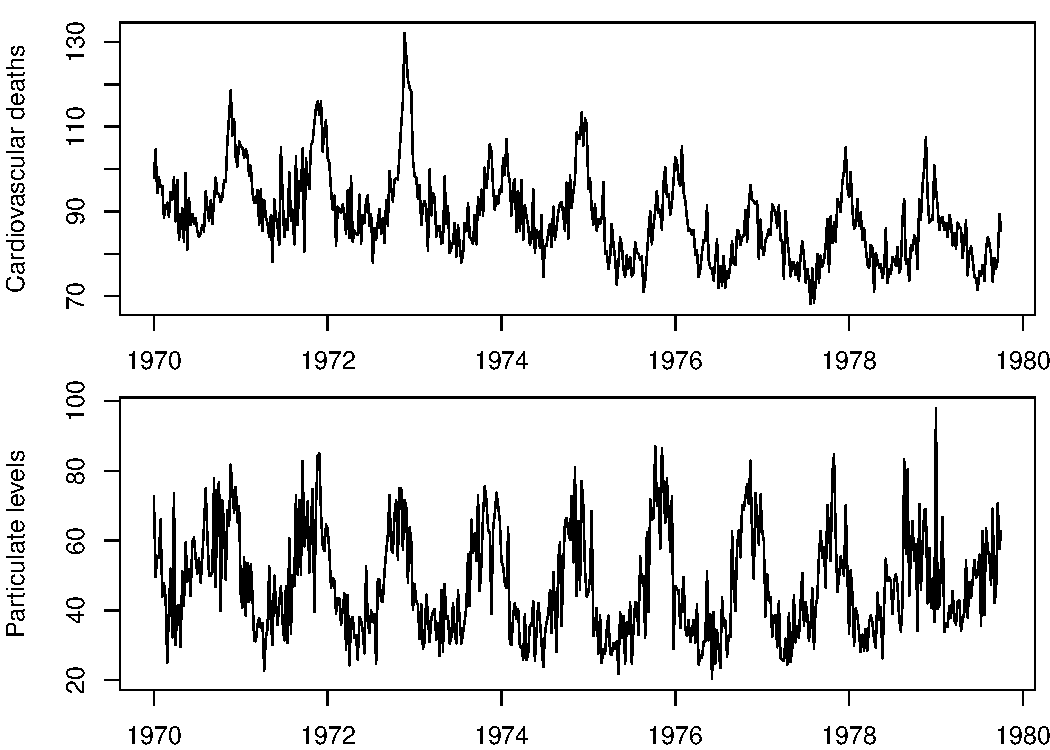
\includegraphics[width=0.875\textwidth]{fig/cardio-1.pdf} 

\bigskip\bigskip
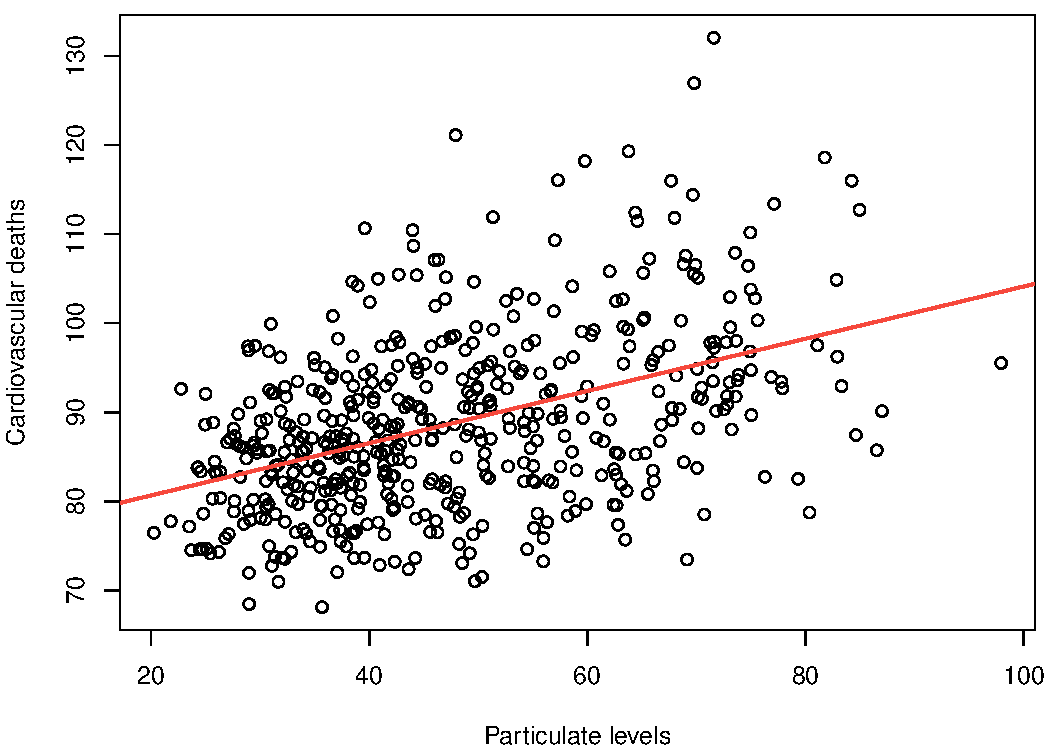
\includegraphics[width=0.875\textwidth]{fig/cardio-2.pdf}

\caption{\it Linear regression of cardiovascular mortality on particulate levels 
  in Los Angeles (from SS).} 
\label{fig:cardio}
\end{figure}
\end{itemize}

\subsection{Prediction: ex-ante and ex-post}

\def\new{\text{new}}

\begin{itemize}
\item We can use the estimated coefficients  \smash{$\hbeta_0, \hbeta_1$} in
  \eqref{eq:beta} from linear regression estimates to make \emph{predictions}
  about the response given a new predictor value $x_{\new}$. This
  prediction is  
  \[
  \hat{y}_{\new} = \hbeta_0 + \hbeta_1 x_{\new},
  \]
  where the ``hat'' notation on the left-hand side emphasizes that it is an not  
  observed, but an estimated (predicted) value of the response

\item In time series context, we often will use the term \emph{forecasting}
  synomously with \emph{prediction}. In the time series, there is an interesting
  distinction between two types of forecasts, based on \emph{whether or not the
    predictor value $x_{\new}$ needed to make forecasts is available in
    advance}. Specifically:   
  \begin{itemize}
  \item An \emph{ex-ante forecast} is a ``true'' forecast, using only
    information that is available at the time the forecast was issued. So the
    predictor values need to either be available, or themselves be
    forecasted. For instance, we can make ex-ante forecasts in the chicken 
    regression example

  \item An \emph{ex-post forecast} is made using later information on the
    predictors. So we wait until $x_{\new}$ is observed, then issue our
    forecast. For instance, we can make ex-post forecasts in the mortality
    regression example (but cannot easily make ex-ante forecasts unless we 
    somehow could forecast particulate levels into the future)
  \end{itemize}

\item One way around the circumvent the potential difficulty of making ex-ante
  forecasts is to use \emph{lagged predictors}; we'll discuss this and other
  forecasting issues in more detail later
\end{itemize}

\subsection{A note on assumptions and philosophy}

\begin{itemize}
\item What have we assumed above? \emph{Nothing.} That is, \emph{we do  
    not need to assume that the true relationship between $y$ and $x$ is linear
    in order to perform linear regression as in \eqref{eq:beta}}

\item Thus, in general, there need not be any ``true regression coefficients'' 
  that we're actually tracking ... but, we can always think of the sample
  estimates \smash{$\hbeta_0, \hbeta_1$} in \eqref{eq:beta} as tracking 
  the population quantities \smash{$\beta^*_0, \beta^*_1$} in
  \eqref{eq:beta_pop}. The latter are basically also always well-defined, 
  regardless of linearity. Recall, they are the viewed as the best linear
  approximation at the population level 

\item So, to be clear, we can always fit sample coefficients \smash{$\hbeta_0,
    \hbeta_1$} and use them to make predictions (forecasting, in time
  series). Sometimes we call this our ``working model'': to use a linear working
  model is a modeling decision, not an assumption  

\item If this predicts well (has good accuracy), then our working model was a
  good decision, and depending on our use case, we may not even care about
  whether the true model is linear (or related assumptions in classical linear
  modeling) 

\item Meanwhile, for use cases would that require \emph{inference}, we require
  lots of assumptions. More, later
\end{itemize}

\section{Multiple regression}

\subsection{Population version}

\begin{itemize}
\item What about the case where we have more than out covariate? This is called
  \emph{multiple linear regression}. Now let $x = (x_1, \dots, x_p) \in \R^p$
  be a random vector of covariates, with each entry $x_j$ being an individual
  covariate of interest

\item We seek $\beta_0$, which is an intercept term as before, and also a whole 
  coefficient vector $\beta = (x_1, \dots, x_p) \in \R^p$, such that 
  \[
  y \approx \beta_0 + \underbrace{\beta_1 x_1 + \cdots + \beta_p
    x_p}_{\textstyle \begin{array}{c} \beta^\T x \end{array}}
  \]

\item Our convention throughout this class will be to \emph{treat all vectors as 
    column vectors}. Thus $a^\T$, which is the transpose of a vector $a$, is a
  row vector, and for vectors $a,b \in \R^d$, we can use $a^\T b = a_1 b_1 +
  \cdots a_d b_d$ to denote their inner product. 

\item (Note that of course $a^\T b = b^\T a$, so it doesn't matter whether we
  write $\beta^\T x$ or $x^\T \beta$ in our model)

\item As in \eqref{eq:ls_pop}, we define the population-level regression
  coefficients by minimizing expected squared error,   
  \begin{equation}
  \label{eq:ls_pop_mult}
  \min_{\beta_0, \beta} \, \E\big[ (y - \beta_0 - x^\T \beta)^2 \big]
  \end{equation}

\item The solution, which you can think of as generalizing \eqref{eq:beta_pop},
  is 
  \begin{equation}
  \label{eq:beta_pop_mult}
  \beta^* = \Cov(x)^{-1} \Cov(x, y), \quad 
  \beta^*_0 = \E(y) - \E(x)^\T \beta^*
  \end{equation}

\item Let's check that the dimensions make sense: here $\Cov(x) \in \R^{p
    \times  p}$, a $p \times p$ matrix of real values; the element in its $i\th$
  row and $j\th$ column is   
  \[
  [\Cov(x)]_{ij} = \Cov(x_i, x_j)
  \]
  Also $\Cov(x, y) \in \R^p$, a $p$-dimensional vector, with $i\th$ entry
  \[
  [\Cov(x, y)]_i = \Cov(x_i, y)
  \]
  So $\Cov(x)^{-1} \Cov(x, y) \in \R^p$, itself a $p$-dimensional vector, which
  is what we need for $\beta^*$ in \eqref{eq:beta_pop_mult}. Similarly, you can
  check that the dimensions make sense for $\beta^*_0$ 

\item To derive \eqref{eq:beta_pop_mult} as the minimizer in
  \eqref{eq:ls_pop_mult}, we can again differentiate with respect to each
  $\beta_j$ and set the result to zero, but the calculation is a little more
  difficult (this is a bonus on the homework) 
\end{itemize}

\subsection{Sample version}

\begin{itemize}
\item The sample version of multiple linear regression falls out of the 
  population version entirely analogously, as it did in the simple linear
  regression case. We seek $\beta_0 \in \R$ and $\beta_1 \in \R^p$ 
  such that for given samples $x_i,y_i$ (covariate and response pairs), $i =
  1,\dots,n$,  
  \[
  y_i \approx \beta_0 + \underbrace{\beta_1 x_{i1} + \cdots + \beta_p 
    x_{ip}}_{\textstyle \begin{array}{c} x_i^\T \beta \end{array}}, \quad 
  i = 1,\dots,n 
  \]

\item We can do this either by plug-in estimates from \eqref{eq:beta_pop_mult},
  or by writing down a sample version of the least squares problem
  \eqref{eq:ls_pop_mult} and solving it, and again they will both lead to the 
  same answer

\item Let's pursue the latter. It will be convenient to adopt the following
  convention, which alleviates us from keeping track of an explicit intercept 
  term $\beta_0$, without any loss of generality. We simply write  
  \[
  y_i \approx x_i^\T \beta, \quad i = 1,\dots,n
  \]
  without intercept. Then all results that we will derive can be translated to
  the model with intercept via the following trick: we redefine each vector
  $x_i$ so that it has a 1 prepended to it:   
  \begin{equation}
  \label{eq:x_intercept}
  x = (1, x_1, \dots, x_p)
  \end{equation}
  Then we read of results in this new parametrization: post-transformation, the
  first entry of $\beta$ serves as the intercept, and the rest serve as the
  coefficients multiplying each $x_j$   

\item (There is another way to get rid of the intercept as well, which we'll
  learn when we connect multiple to simple linear regression a bit later, which
  may be more intuitive to some of you) 

\item The sample least squares problem for multiple regression is now as
  follows:  
  \begin{equation}
  \label{eq:ls_mult1}
  \min_{\beta \in \R^p} \, \sum_{i=1}^n (y_i - x_i^\T \beta)^2 
  \end{equation}

\item The solution, obtained again by taking derivatives and setting equal to
  zero, is
  \begin{equation}
  \label{eq:beta_mult1}
  \hbeta = \bigg( \sum_{i=1}^n x_i x_i^\T \bigg)^{-1} \sum_{i=1}^n x_i y_i  
  \end{equation}

\item You can check that the dimensions all make sense here (that the right-hand
  side in \eqref{eq:beta_mult1} produces the correct dimensions for
  \smash{$\hbeta$}) 
\end{itemize}

\subsection{Matrix notation}

\begin{itemize}
\item It is more convenient, once you've sufficiently familiarized yourself with
  matrix notation, to recast regression in terms of matrices and vectors. Let $y 
  = (y_1, \dots, y_n) \in \R^n$ be the vector of our response values, and $X \in
  \R^{n \times p}$ the matrix of our predictor vectors, whose $i\th$ row is
  $x_i^\T$    

\item In other words,
  \[
  y = \begin{bmatrix} 
    y_1 \\ y_2 \\ \vdots \\ y_n 
  \end{bmatrix}, \quad 
  X = \begin{bmatrix} 
    x_{11} & x_{12} & \cdots & x_{1p} \\
    x_{21} & x_{22} & \cdots & x_{2p} \\
    \vdots & & & \\
    x_{n1} & x_{n2} & \cdots & x_{np} 
    \end{bmatrix}
  \]

\item Recall, for a coefficient vector $\beta \in \R^p$, the matrix-vector
  product $X \beta \in \R^n$, which to emphasize is an $n$-dimensional vector,
  is    
  \[
  X \beta = 
  \begin{bmatrix} 
    x_1^\T \beta \\ x_2^\T \beta \\ \vdots \\ x_n^\T \beta 
  \end{bmatrix}
  \]
  This means that we can write our sample working model compactly as
  \[
  y \approx X \beta
  \]

\item Recall, the Euclidean or $\ell_2$ norm $\|\cdot\|_2$ of a vector $a \in
  \R^d$ is defined as \smash{$\|a\|_2^2 = \sum_{i=1}^d a_i^2$}. This means we
  can write our sample least squares problem \eqref{eq:ls_mult1} compactly as  
  \begin{equation}
  \label{eq:ls_mult2}
  \min_{\beta \in \R^p} \, \|y - X \beta\|_2^2
  \end{equation}

\item Finally, the sample least squares estimates \eqref{eq:beta_mult1} can 
  be written as 
  \begin{equation}
  \label{eq:beta_mult2}
  \hbeta = (X^\T X)^{-1} X^\T y  
  \end{equation}
  This form \eqref{eq:beta_mult2} is by far the more commonly-used (and
  easily-remembered) form for the least squares coefficient estimates, compared
  to \eqref{eq:beta_mult1}. You'll prove the equivalence between the two
  forms \eqref{eq:beta_mult1}, \eqref{eq:beta_mult2} on the homework 

\item Important technical note: above in \eqref{eq:beta_mult2} (also in
  \eqref{eq:beta_mult1}), we have implicitly assumed that the features---the 
  columns of $X$---are \emph{linearly independent}. This \emph{can only happen
    if $p \leq n$}, i.e., if we have no more features than samples. Otherwise,
  $X^\T X$ will not have an inverse, strictly speaking. This is not the end of
  the world and there are many interesting things to talk about (along the lines
  of regularization) when $p > n$, but it's beyond our scope in these notes. 
  More, next time! 
\end{itemize}

\subsection{Multiple vs simple: a connection}

\begin{itemize}
\item There is quite an interesting connection between multiple regression of
  $y$ on $x$ and simple regression of $y$ on each $x_j$, the latter often
  referred to as a \emph{marginal linear regression}

\begin{quote}\it
**Warning** 

There will be a notational clash between $x_i$ as used above and $x_j$ as will
be used here. Previously, we used $x_i \in \R^p$ to refer to vector containing
all feature values for the $i\th$ sample. Here, we are going to use $x_j \in
\R^n$ to refer to the vector containing the $j\th$ feature values measured over
all samples.       

For example, suppose we have two features: apples and bananas, and we measure
the quantity of each across $n = 100$ households. Then the previous subsection
used $x_i \in \R^2$ as the number of apples and bananas in the $i\th$
household. But here we'll use $x_j \in \R^{100}$ as the number of apples (if
$j=1$) in the 100 households, or bananas (if $j=2$) in the households. Get it? 

Since the beginning of \sout{time} regression, scholars have run up against this
problem and have racked their brains for notational solutions. But there is no
real good notational solution to this. (Yes there are lots of options but all of
them have some ugliness to them.)

We'll just make to use $x_i \in \R^p$ to \emph{always} refer to all features for
the $i\th$ sample, and $x_j \in \R^n$ to \emph{always} refer to the the $j\th$
feature for all samples (and try to never mix indices). In other words, the
$i\th$ row and $j\th$ column of the feature matrix $X$, respectively. So you
just have to remember that $i$ indexes samples (rows), and $j$ indexes features
(columns). 

**End warning** 
\end{quote}

\item Now that we've gotten that important notational piece out of the way, we
  will define more quantities in order to describe the connection between
  multiple and marginal regression

\item Fix any $j$ (arbitrary). Given a single feature $x_j = (x_{1j}, \dots,
  x_{nj}) \in \R^n$, and response vector $y = (y_1, \dots, y_n) \in \R^n$, the 
  marginal (or simple) regression of $y$ on $x_j$, \emph{without intercept}, is
  a very similar formula to what you saw in \eqref{eq:beta}:
  \[
  \tilde\beta_j = \frac{\sum_{i=1}^n x_{ij} y_i}{\sum_{i=1}^n x_{ij}^2} 
  \]
  (Note: the effect of the intercept is only that it centers the values of
  $x_{ij}$ around their sample average, and $y_i$ around their sample average)     

\item We can rewrite this succinctly in inner product notation as:
  \begin{equation}
  \label{eq:beta_j}
  \tilde\beta_j = \frac{x_j^\T y}{x_j^\T x_j}
  \end{equation}

\item Meanwhile, let's consider the $j\th$ estimated regression coefficient
  $\hbeta_j$ from the multiple regression of $y$ on $X$, as in
  \eqref{eq:beta_mult2}. Is this the same? That is, is the $j\th$ component of
  \eqref{eq:beta_mult2} the same as \eqref{eq:beta_j}? 

\item The answer is generally no! Putting in other features into the linear
  regression will generally affect the estimated coefficient for $x_j$, i.e.,
  will alter its ``predictive influence'' on $y$

\item However, there is a precise connection between multiple regression and
  marginal regression. Let's write $X_{-j} \in \R^{n \times p}$ for the feature
  matrix but after dropping $x_j \in \R^n$, the $j\th$ column. Suppose we:  
  \begin{itemize}
  \item Regress $y$ on $X_{-j}$ (a regression of $y$ on all but the $j\th$
    feature), yielding an estimated coefficient vector \smash{$\halpha \in
      \R^{p-1}$}, and residual  
    \begin{equation}
    \label{eq:resid_y}
    \hat{y}^{-j} = y - X_{-j} \, \halpha 
    \end{equation}

  \item Regress $x_j$ on $X_{-j}$ (a regression of $x_j$ on all of the other
    features), yielding an estimated coefficient vector \smash{$\htheta \in 
      \R^{p-1}$}, and residual  
    \begin{equation}
    \label{eq:resid_j}
    \hat{x}^{-j}_j = x_j - X_{-j} \, \htheta 
    \end{equation}
  \end{itemize}

\item In these residuals \eqref{eq:resid_y}, \eqref{eq:resid_j}, we have
  ``regressed out the influence'' of all other features on each of $y$ and
  $x_j$. Then, after removing such infuence, if we perform a marginal regression
  of \smash{$\hat{y}^{-j}$} on \smash{$\hat{x}^{-j}_j$}, we get precisely the
  $j\th$ multiple regression coefficient: 
  \begin{equation}
  \label{eq:beta_j_mult}
  \hbeta_j = \frac{(\hat{x}^{-j}_j)^\T\hat{y}^{-j}}
  {(\hat{x}^{-j}_j)^\T\hat{x}^{-j}_j} 
  \end{equation}

\item In other words, \eqref{eq:beta_j_mult} connects multiple regression to
  marginal regression: it shows that the $j\th$ coefficient in a multiple
  regression \eqref{eq:beta_mult2} is equivalent to a marginal regression of $y$
  on $x_j$, but only after we have accounted for the effects of all the other
  predictors, by ``regressing them out'' 

\item The best way to understand the relationship between \eqref{eq:beta_j_mult}
  and \eqref{eq:beta_mult2} is geometrically (which is also a great way to view 
  linear regression in general) but that perspecive requires a bit more advanced
  linear algebra, which we won't cover. For now, you can just think of the
  following: the bigger the \emph{correlations} between $x_j$ and columns of
  $X_{-j}$, the bigger the effect will be in \eqref{eq:resid_j}, where we
  regress out $X_{-j}$ from $x_j$, and this will make the multiple
  \eqref{eq:beta_j_mult} and marginal \eqref{eq:beta_j} coefficients quite 
  different from each other

\item On the other hand, when $x_j$ is orthogonal to (or uncorrelated with, if
  we are using a model with intercept) each column of $X_{-j}$, then the
  residual \smash{$\hat{x}^{-j}_j$} in \eqref{eq:resid_j} is no different from
  $x_j$, and in fact one can show that the multiple regression coefficient in
  \eqref{eq:beta_j_mult} and the marginal one in \eqref{eq:beta_j} are the same    

\item Figure \ref{fig:cardio_mult} revisits the cardiovascular mortality example
  from earlier. Now we perform the regression of cardiovascular mortality on two
  features: particulate levels and temperature. (In R we can regress \verb|y| on
  two features \verb|x1| and \verb|x2| by running \verb|lm(y ~ x1 + x2)|.) For
  each feature, the coefficients from multiple regression aren't too different
  from the marginal regression coefficients (as is seen in the bottom panel by
  the slopes of the lines), though the intercept changes noticeably. The 
  relatively small change in the coefficients on particulate levels and
  temperature is due to the fact that these two are not very correlated (as is
  seen by looking at their time series, which are a bit ``out of phase'' with
  each other) 

\begin{figure}[p]
\centering
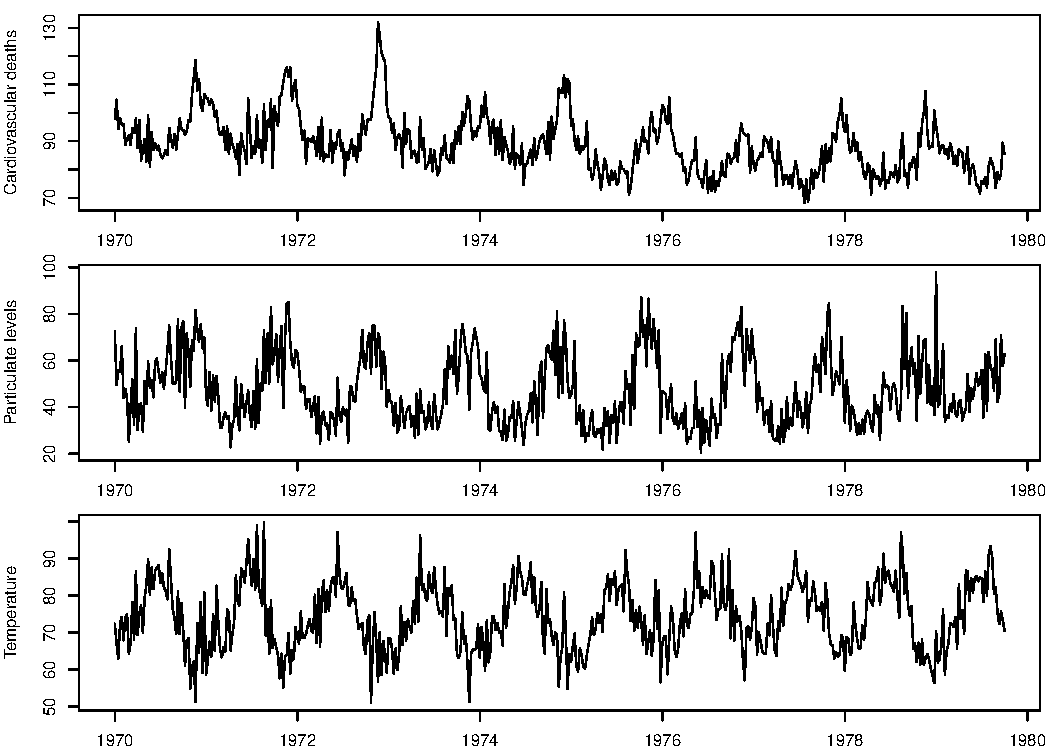
\includegraphics[width=0.875\textwidth]{fig/cardio-mult-1.pdf} 

\bigskip\bigskip
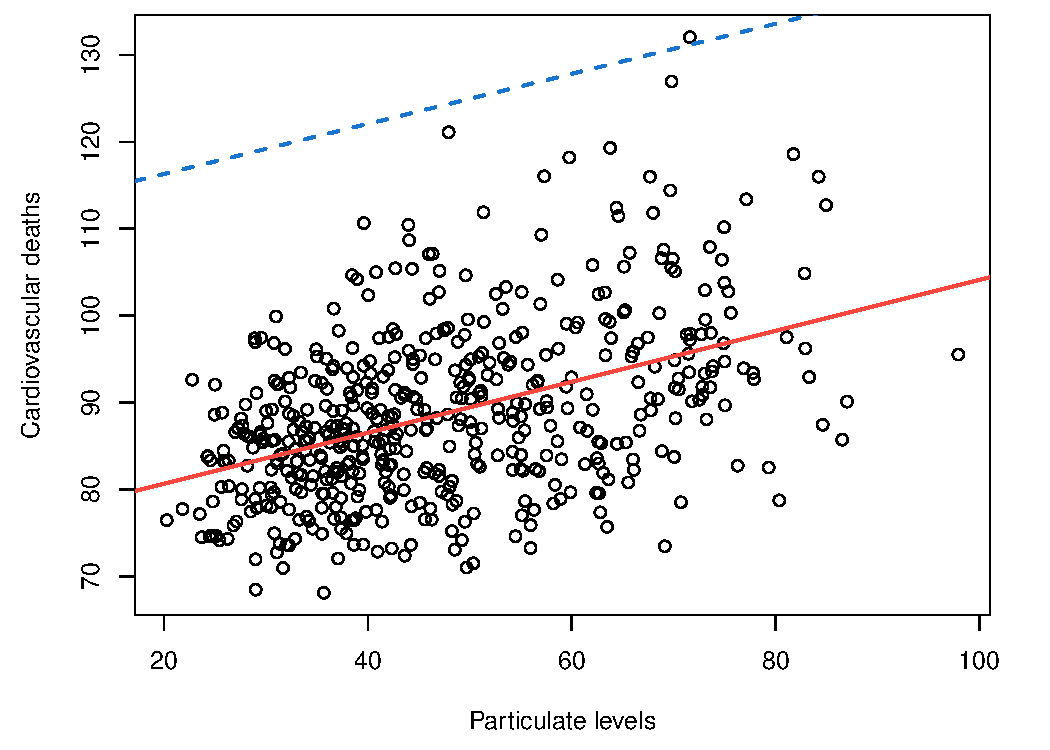
\includegraphics[width=0.475\textwidth]{fig/cardio-mult-2.pdf}
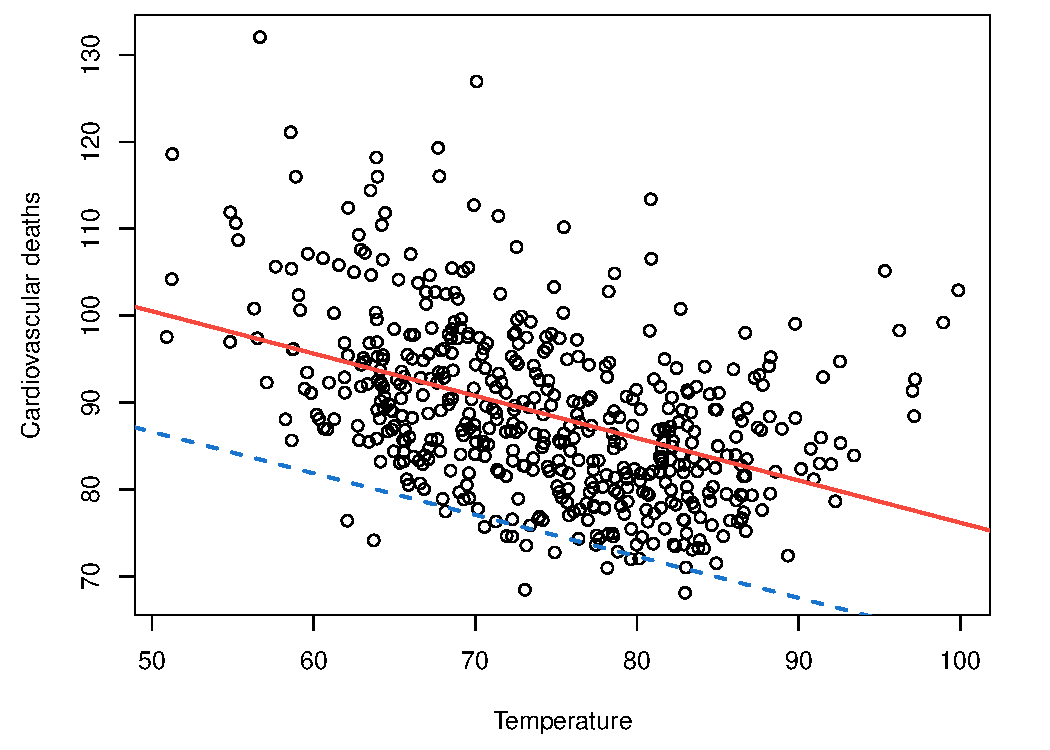
\includegraphics[width=0.475\textwidth]{fig/cardio-mult-3.pdf}

\caption{\it Linear regression of cardiovascular mortality on particulate levels
  and temperature (this is multiple regression, with two features) in Los
  Angeles (from SS). The solid red lines denote the estimates from marginal
  regression; the dashed blue from multiple regression.} 
\label{fig:cardio_mult}
\end{figure}
\end{itemize}

\subsection{Interlude: best linear unbiased estimator}

\def\WN{\mathrm{WN}}
\def\MSE{\mathrm{MSE}}

\begin{itemize}
\item Briefly, we discuss an important optimality property here of least squares
  estimates, before moving on to classical inferential results next. We are
  going to need to introduce an assumption for this part: we assume that the
  response vector $y \in \R^n$ is related to the feature matrix $X \in \R^{n
    \times p}$ by
  \begin{equation}
  \label{eq:model_wn}
  y = X \beta + \epsilon, \quad \text{where $\epsilon \sim \WN(0, \sigma^2 I)$}   
  \end{equation}
  for some unknown coefficient vector $\beta \in \R^p$, and a white noise vector 
  $\epsilon \in \R^n$

\item In \eqref{eq:model_wn}, $\epsilon \sim \WN(0, \sigma^2 I)$ is our notation
  for a white noise vector: the first argument specifies that the mean is zero, 
  $\E(\epsilon) = 0$, and the second argument specifies that the covariance
  satisfies $\Cov(\epsilon) = \sigma^2 I$, where $I$ is the $n \times n$
  identity matrix. That is, the components satisfy $\Var(\epsilon_i) = \sigma^2$
  and $\Cov(\epsilon_i, \epsilon_j) = 0$ whenever $i \not= j$

\item Importantly, in \eqref{eq:model_wn}, the feature matrix $X$ is assumed to
  be \emph{fixed} (not random). Therefore, we can also write \eqref{eq:model_wn}
  even more compactly as 
  \[
  y \sim \WN(X \beta, \sigma^2 I)
  \]

\item Assuming that $X$ is fixed in the context of the above model is a fairly
  strong condition. We'll go into more why in the next section (when we go even 
  further and assume normality of the error distribution), but for now we'll
  just emphasize that we are assuming that the mean of the response is truly
  linear in the features, and that the errors are homoskedastic---they have
  equal variance regardless of the feature values 

\item Ok! So under the model \eqref{eq:model_wn}, what can we say about the
  least squares estimates in \eqref{eq:beta_mult2}? First, note that these are 
  \emph{unbiased} for the true coefficients $\beta$:
  \begin{align*}
  \E(\hbeta) &= \E \big[ (X^\T X)^{-1} X^\T y \big] \\
  &= (X^\T X)^{-1} X^\T \E(y) \\
  &= (X^\T X)^{-1} X^\T X \beta \\
  &= \beta
  \end{align*}

\item This implies it is unbiased for any contrast of $\beta$. This is the term 
  we sometimes give to an estimand of the form $a^\T\beta$, for an 
  arbitrary vector $a \in \R^d$. Observe, 
  \[
  \E(a^\T \hbeta) = a^\T \E(\hbeta) = a^\T \beta
  \]

\item One common way to measure the quality of an estimator is its \emph{mean
    squared error} (MSE), which for the least squares estimator \smash{$a^\T
    \hbeta$} of the contrast $a^\T \beta$, is
  \[
  \MSE(a^\T \hbeta) = \E\big[ (a^\T \hbeta - a^\T \beta)^2 \big]
  \]
  To be clear, the expectation here is being taken with respect to data from the
  model \eqref{eq:model_wn} 

\item With respect to MSE, how good is the least squares estimator? It is, in a
  certain precise sense, the \emph{best}. It is both unbiased for $a^\T \beta$,
  as proved above, and also a \emph{linear} estimator as a function of $y$: we
  can write  
  \[
  a^\T \hbeta = \underbrace{(a^\T X^\T X)^{-1}
    X^\T}_{\textstyle \begin{array}{c} b^\T \end{array}} y  
  \]
  That is, $a^\T \hbeta = b^\T y$, where $b = X (X^\T X)^{-1} a$ 

% \item We could have also done this more explicitly from the equivalent
%   formulation in \eqref{eq:beta_mult1}:
%    \begin{align*}
%   a^\T \hbeta &= a^\T \bigg( \sum_{i=1}^n x_i x_i^\T \bigg)^{-1} \sum_{i=1}^n
%                 x_i y_i \\ 
%   &= \sum_{i=1}^n \underbrace{a^\T \bigg( \sum_{i=1}^n x_i x_i^\T \bigg)^{-1} 
%     x_i}_{\textstyle \begin{array}{c} b_i \end{array}} y_i 
%   \end{align*}
%   That is, $a^\T \hbeta \sum_{i=1}^n b_i y_i$, where \smash{$b_i = a^\T (
%     \sum_{i=1}^n x_i x_i^\T )^{-1} x_i$}, which is the same thing just written
%   differently 

\item Note: linearity of the estimator has nothing to do with linearity of the
  true regression model! The former (linearity of the estimator) is a statement
  about linearity in $y$, the response; the latter (linearity of the true
  regression model) is a statement about linearity in $X$, the features. This
  is a nomenclature collision, and linearity is really referring to different
  things here 

\item Now for the main event: the \emph{Gauss-Markov theorem} tells us that
  the least squares estimator is the best linear unbiased estimator (BLUE) of
  $a^\T \beta$. In other words, for any other linear estimator $c^\T y$, such
  that $\E(c^\T y) = a^\T \beta$ (unbiasedness), we have  
  \[
  \MSE(a^\T \hbeta) \leq \MSE(c^\T y)
  \]

\item A proof of this fact follows from the geometric perspective on least
  squares, which we won't cover, but you can ask about it in office hours if you
  are curious  

\item (An interesting side note! Econometricians have been recently arguing about 
  whether or not we can drop the ``L'' from BLUE: is least squares the BUE? That
  is, is least squares the best unbiased estimator, period---best among all
  unbiased estimators, not just linear ones? The answer is ... yes, in a sense,
  but it depends on how you set up the problem, because in certain problem
  settings the only unbiased estimators are linear in $y$ anyway!\footnote{See
    Hansen (2022), ``A modern Gauss-Markov theorem'', and then P{\"o}tscher and
    Preinerstorfer (2022), ``A modern Gauss-Markov theorem? Really?'', and then
    Portnoy (2022), ``Linearity  of unbiased linear model estimators''. A nice
    and friendly overview is given by Allison (2022), ``Is OLS BLUE or BUE?'',
    \url{https://statisticalhorizons.com/is-ols-blue-or-bue/} (this is a blog
    post). A masterful, but much more mathematical treatment is given in Lei and
    Wooldrige (2022), who also weave in important historical results that seem
    to have been overlooked, and prove new ones as well.})  
\end{itemize}

\section{Classical inference}

\subsection{Here comes the assumptions}

\def\iidsim{\overset{\text{iid}}{\sim}}

\begin{itemize}
\item Now we're going to cover some classical statistical inference for linear
  regression estimates. For this part, we're going to need to assume:
  \begin{equation}
  \label{eq:model_n}
  y = X \beta + \epsilon, \quad \text{where $\epsilon \sim N(0, \sigma^2 I)$}
  \end{equation}
  In comparison to \eqref{eq:model_wn}, note that we have additionally assumed
  that the errors are multivariate Gaussian (this implies they are independent
  across observations as well)

\item As before, the feature matrix $X$ is assumed to  be \emph{fixed} (not
  random). Thus we can write \eqref{eq:model_n} more compactly as  
  \[
  y \sim N(X \beta, \sigma^2 I)
  \]

\item Taking $X$ to be fixed here is a strong assumption. To see this, let's
  write this out as 
  \[
  y_i = x_i^\T \beta + \epsilon_i, \quad \text{where $\epsilon_i \iidsim N(0,  
  \sigma^2)$}, \quad i=1,\dots,n
  \]
  If each $x_i$ were indeed random (which is often the case in practice) then we
  would need \emph{condition on $x_i$} in order to treat it as fixed. So then,
  what the above model really says is that each $\epsilon_i | x_i$ is normal
  with mean zero and variance $\sigma^2$. And for this to be true across all 
  observations, we need the \emph{errors $\epsilon_i$ and feature vectors $x_i$
    to be independent}

\item Now we have gotten to the heart of why this is such a strong
  assumption. For the errors and features to be independent, we cannot have
  \emph{heteroskedasticity} (error variance depending on the features); we also
  cannot really have any \emph{omitted variables}, because if they are
  correlated with $x_i$, then they would appear in the effective error term
  $\epsilon_i$, and break independence. Can you really make the argument that
  you have measured \emph{all} of the relevant predictor variables in any given 
  practical application of linear regression? 
\end{itemize}

\subsection{t-test for individual coefficients}

\begin{itemize}
\item Under \eqref{eq:model_n}, we can define a \emph{t-test}, based on the
  least squares estimate \eqref{eq:beta_mult2}, for testing whether or not an 
  individual coefficient is zero at the population-level: that is, for testing
  the hypothesis 
  \begin{equation}
  \label{eq:null1}
  H_0 : \beta_j = 0
  \end{equation}

\item To set us up to discuss this, we first define an estimate of the noise
  variance $\sigma^2$ in \eqref{eq:model_n}:
  \begin{align*}
  \hat\sigma^2 &= \frac{1}{n-p} \|y - X\hbeta\|_2^2 \\ 
  &= \frac{1}{n-p} \sum_{i=1}^n (y_ i - x_i^\T \hbeta)^2 
  \end{align*}
  This is the residual sum of squares from linear regression, divided by $n-p$ 

\item We also define the matrix $C = (X^\T X)^{-1}$. Why is this important?
  Because: 
  \begin{align*}
  \Cov(\hbeta) &= \Cov\big( (X^\T X)^{-1} X^\T y \big) \\
  &= (X^\T X)^{-1} X^\T \Cov(y) X (X^\T X)^{-1} \\
  &=  (X^\T X)^{-1} X^\T \sigma^2 I X (X^\T X)^{-1} \\
  &= \sigma^2 (X^\T X)^{-1} \\
  &= \sigma^2 C
  \end{align*}
  Note: in the second line we the property of covariance: for a random vector
  $z$ and matrix $A$ of appropriate dimension, $\Cov(Az) = A \Cov(z)
  A^\T$. We'll revisit this and related properties on the homework

\item The above result implies that \smash{$\Var(\hbeta_j) = \sigma^2 C_{jj}$},
  where $C_{jj}$ is the $j\th$ diagonal element of $C$

\item Recall that we also know that \smash{$\E[\hbeta_j] = \beta_j$}, since we
  already proved unbiasedness, above. Combining two these facts (about the mean 
  and variance of \smash{$\hbeta_j$}) leads us to define the \emph{t-statistic}  
  \begin{equation}
  \label{eq:t_stat}
  t_j = \frac{\hbeta_j}{\hat\sigma \sqrt{C_{jj}}} 
  \end{equation}
  Under \eqref{eq:model_n}, this is has a \emph{t-distribution} with $n-p$
  degrees of freedom. This can be used to test \eqref{eq:null1}, or a similar
  construction can be used form a confidence interval for $\beta_j$. This
  follows the same general recipe that you have learned (or will learn) about
  hypothesis testing and confidence intervals in your concepts of statistics
  class 

\item When you call \verb|lm()| in R, and then call \verb|summary()| on its
  output, you are presented with these t-statistics and associated p-values (for
  the test that the coefficient is zero, as in \eqref{eq:null1})

\item We will not cover this further, in any real detail, because (a) you'll
  likely spend a good amount of time on this when you learn regression in your
  concepts of statistics course, and (b) we won't really rely on classical
  inferential tools such as this t-test very much. After all, they rest on the
  assumption that the model \eqref{eq:model_n} is correct, which (as we've
  discussed already) can be a dubious one in practice
\end{itemize}

\subsection{F-test for subgroups of coefficients}

\def\SSE{\mathrm{SSE}}

\begin{itemize}
\item Even more briefly, we can form an \emph{F-test} for the hypothesis that an
  entire \emph{group} of coefficients is zero, which (with a loss of generality,
  just by relabeling the features), we can write as
  \begin{equation}
  \label{eq:null2}
  H_0 : \beta_{k+1} \cdots = \beta_p = 0
  \end{equation}

\item We define
  \[
  \SSE = \sum_{i=1}^n (y_i - x_i^\T \hbeta)^2, \quad \text{and} \quad 
  \SSE(k) = \sum_{i=1}^n \big( y_i - x_i^\T \hbeta(k) \big)^2
  \]
  where \smash{$\hbeta(k) \in \R^k$} denotes the estimated regression
  coefficients when only the first $k$ features are present

\item We then define the \emph{F-statistic}  
  \begin{equation}
  \label{eq:f_stat}
  F_k = \frac{(\SSE(k) - \SSE) / (p-k)}{\SSE / (n-p)}
  \end{equation}
  Under \eqref{eq:model_n} and \eqref{eq:null2}, this has a \emph{central
    F-distribution} with $p-k$ and $n-p$ degrees of freedom. We can use this to
  test \eqref{eq:null2}, the hypothesis that all but the first $k$ true
  coefficients are zero

\item An important special case: when $k = p-1$, we are testing whether $\beta_p
  = 0$, and it can be shown that the F-statistic $F_p$ in \eqref{eq:f_stat} is
  equivalent to the t-statistic $t_p$ in \eqref{eq:t_stat} for testing $\beta_p
  = 0$, from the previous subsection  
\end{itemize}

\subsection{AIC, BIC, AICc, $R^2$, adjusted $R^2$, ...}

\begin{itemize}
\item We will not cover these. These are classical tools for variable/model
  selection. You can read about them in SS (Chapter 2.1) and/or HA (Chapter 7.5) 
  books if you are interested. We'll take a more predictive angle, and focus
  instead on tools like cross-validation  
\end{itemize}

\subsection{Diagnostics, transformations}

\begin{itemize}
\item There are a variety of diagnostic (statistical) tools for evaluating the
  output of a regression model. One of the most relevant tools to us, in the 
  time series setting, is to examine the auto-correlation function of the 
  residuals   
  \[
  \hat\epsilon_i = y_i - x_i^\T \hbeta, \quad i = 1,\dots,n
  \]
  
\item Recalling \eqref{eq:model_wn}, one of the assumptions underlying the
  theory of linear regression (the Gauss-Markov theorem, t-tests, F-tests, etc.)
  is that the errors $\epsilon_i = y_i - x_i^\T \beta$, $i = 1,\dots,n$ form a 
  white noise sequence  

\item Thus inspecting the auto-correlation function of residuals gives us a
  sense of whether this white noise assumption is true or not

\item Figure \ref{fig:cardio_acf} shows the result for the mortality regression
  example. We see that there are some very clear auto-correlations persisting  
  through about lag 15. This should have us call into question any classical
  inferential tools we may want to apply. However, more constructively, it means
  that we may be able to improve the regression by taking into account the fact
  that there is structure/information left in the residuals. We will revisit
  this when we discuss ARIMA models, later 

\begin{figure}[htb]
\centering
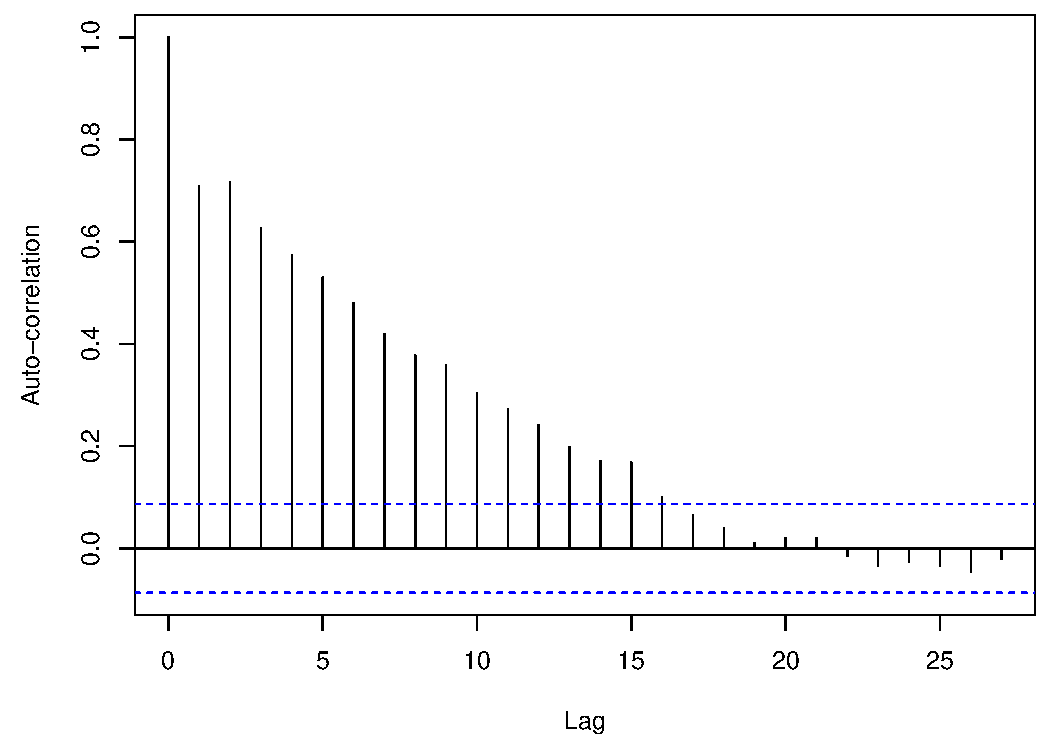
\includegraphics[width=0.875\textwidth]{fig/cardio-mult-4.pdf} 
\caption{Auto-correlation function of the residuals for the linear regression of
  cardiovascular mortality on particulate levels.}
\label{fig:cardio_acf}
\end{figure}

\item Beyond looking at the auto-correlation of the residuals, there are a
  variety of classical diagnostics for regression. You can read about these in 
  many sources, including the R help file for \verb|plot.lm()|, and the HA book
  (Chapter 7.3). We will not be able to cover them, for the sake of time,
  however they are worth being generally aware of, and so worth reading up on
  separately (and/or hopefully you will see them in more detail in another
  course)    

\item Finally, closely related to diagnostics, and another classic topic, are
  transformations--- made either to the response or features---which can improve
  the regression model. We won't cover them for the sake of time, but you can
  look at the HA book for details (Chapters 3.1, 5.6, and 7.4)
\end{itemize}

\subsection{Correlation vs causation?}

\begin{itemize}
\item \emph{Correlation is not causation.} Hopefully that's very clear to you in
  the abstract, and you've been warned of it several times already in previous
  courses

\item However, in the context of regression, it gets a bit murky. Estimation in
  regression is, at its core, about correlation (recall, e.g.,
  \eqref{eq:beta_j_mult}). But causality lurks in the background in the
  interpretation of regression coefficients (which we have purposefully
  avoided), and inferential tools like the t-test for individual coefficients as
  in \eqref{eq:null1}    

\item You have to be very careful to remember that these are predicated on the
  correctness of the model \eqref{eq:model_n} (with fixed $X$). \emph{It is this
    model that allows us to translate statements about correlations to ones that
    look causal.} If this model is wrong (likely!) then these translations break
  down 

\item As already mentioned several times, we are taking a predictive angle and
  will be mostly focused on evaluating models for their utility in prediction,
  or forecasting in time series

\item Fundamentally, \emph{correlations} between variables can be useful for
  forecasting, whether or not they are causal. Everybody would probably agree
  that they'd prefer a simple causal relationship if they could find one; but
  that is a much, much harder problem. Focusing on correlations and predictions
  (and eschewing much of classical inference and interpretation) can be much
  more tractable, in a sense

\item But at the bottom of it all, \emph{``does the model predict well?''} is
  simply a different question. And it may not be the question that you want to
  answer in every application, so having inference tools in your toolkit,
  understanding when they are valid, and learning about causality, will make you
  a more well-rounded statistician
\end{itemize}

\section{Prediction}

\subsection{Lagged predictors}

\begin{itemize}
\item In certain situations, as discussed above, ex-ante forecasts may be
  difficult to obtain. Recall that in the cardiovascular mortality regression 
  example, where $y_t$ is the number of cardiovascular deaths at time $t$ and
  $x_t$ is the level of particulate matter at time $t$, a forecast of mortality
  \smash{$\hat{y}_{t+k}$} at time $t+k$ would only be possible given the
  particulate level $x_{t+k}$ at time $t+k$, which is not available in advance  

\item One way around this is use \emph{lagged predictors} in the regression,
  i.e., instead of regressing $y_t$ on $x_t$, we regress $y_t$ on $x_{t-k}$,
  i.e., we regress deaths each week on particulate levels $k$ weeks earlier:
  \[
  y_t \approx \beta_0 + \beta_1 x_{t-k}, \quad t = 1,2,3,\dots
  \]

\item In doing so, we can make predictions up to $k$ weeks into the future. To
  be clear, if we've only observed data up through time $t$, then we can still
  make forecasts
  \[
  \hat{y}_{t+i} = \hbeta_0 + \hbeta_1 x_{t+i-k}, \quad i = 1,\dots,k
  \]

\item Figure \ref{fig:cardio_lagged} gives an example where we do so with $k =
  4$. We are therefore able to make true, ex-ante forecasts 4 weeks past the end
  of the time series. However, we are not able to validate these, since don't
  actually have data past the summer of 1979 in this example 

\begin{figure}[htb]
\centering
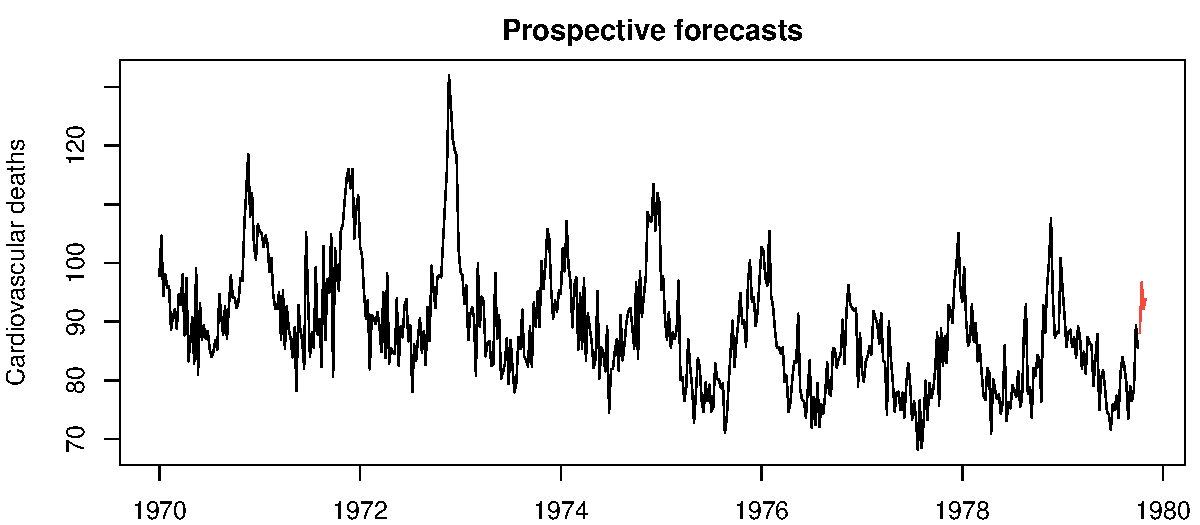
\includegraphics[width=0.9\textwidth]{fig/cardio-lagged-1.pdf} 
\caption{Forecasts of cardiovascular mortality made at a 4-week ahead horizon,
  using particulate level as a lagged predictor. These are prospective
  forecasts, made at the end of the time series.}
\label{fig:cardio_lagged}

\bigskip
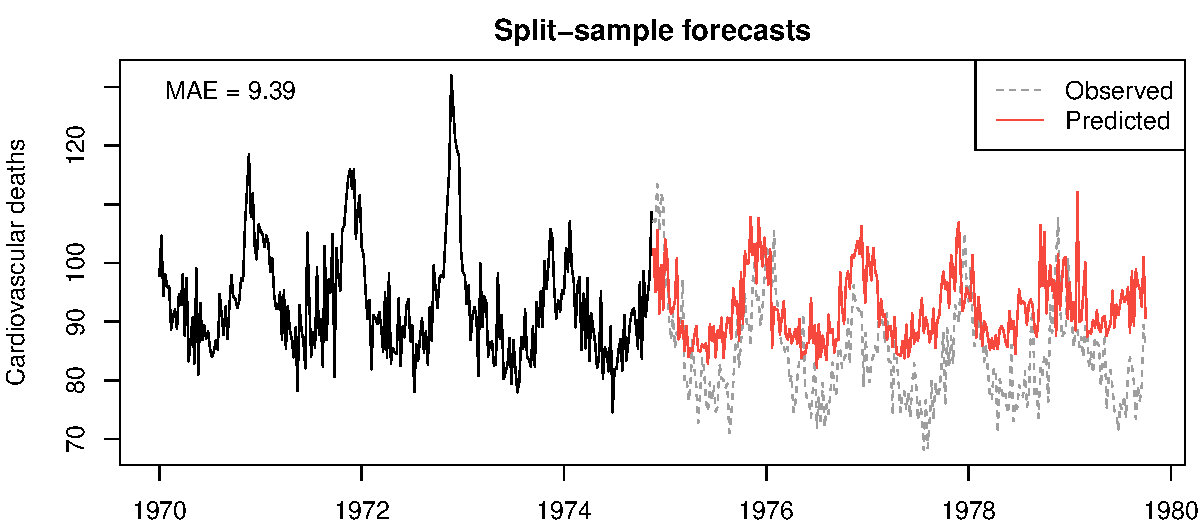
\includegraphics[width=0.9\textwidth]{fig/cardio-split-1.pdf} 

\caption{As in the above figure, but pseudo-prospective forecasts on the second
  half, from a regression model fit only to the first half.} 
\label{fig:cardio_split}
\end{figure}

\item As validation, we can refit the lagged regression on the first half of the
  time series, and use the second half to 4-week ahead make forecasts and
  compare them to the observed series. This is done in Figure
  \ref{fig:cardio_split}. It looks OK in terms of its \emph{dynamics}: the trend
  (rise and fall) in the predictions matches the observed trend fairly well, but
  pretty soon it appears to be biased upwards, particularly at the trough of
  each yearly cycle  

\item (A word of warning: pulling this off correctly in R is actually more
  tricky than you might expect, so study the code in the R notebook carefully
  ...)   

\item Of course, we can also use more than one lag as a predictor, and use as
  our working model:
  \[
  y_t \approx \beta_0 + \sum_{j=1}^m \beta_j x_{t-k_j}, \quad t = 1,2,3,\dots
  \]
  for lags $k_1 < \cdots < k_m$. Note that this model would allow us to make
  forecasts $k_1$ time steps into the future (a lagged predictor model is
  limited by its smallest lag)

\item The more lags---the more features, in general---that we include in the
  working model, the more \emph{expressive} it is, meaning, it is able to
  capture and propogate more intricate trends. But also, the more
  \emph{volatile} it can become, meaning, it can make more wild predictions 

\item Thus there is a tradeoff here, often referred to as the
  \emph{bias-variance tradeoff}. More expressive = lower bias, more volatile =
  higher variance. This tradeoff generally expresses itself differently in
  different problems, and is not something we can anticipate precisely in
  advance. However, fortunately, we can still use generic tools like
  cross-validation to estimate prediction error (which measures bias and
  variance in aggregate). We will cover this next

\item Another important general tool to mention is regularization, which can
  often tilt the bias-variance tradeoff in our favor. We will also cover this
  shortly 
\end{itemize}

\subsection{Error metrics}

\def\MSE{\mathrm{MSE}}
\def\MAE{\mathrm{MAE}}
\def\MAPE{\mathrm{MAPE}}
\def\MASE{\mathrm{MASE}}

\begin{itemize}
\item To evaluate regression models for their predictive accuracy, we'll first
  have to talk about error metrics: the precise formulae we will be using to 
  measure this. The most common one is mean squared error (MSE) between  
  predictions \smash{$\hat{y}_{\text{new},t}$} and unseen observations
  \smash{$y_{\text{new},t}$}, over test times $t = 1,\dots,N$:
  \[
  \MSE = \frac{1}{N} \sum_{t=1}^N \big( y_{\text{new},t} -
  \hat{y}_{\text{new},t} \big)^2
  \]

\item Another common one is mean absolute error (MAE), which tends to focus less
  on extreme errors: 
  \[
  \MAE = \frac{1}{N} \sum_{t=1}^N \big| y_{\text{new},t} -
  \hat{y}_{\text{new},t} \big|
  \]

\item Note that MSE and MAE are scale-dependent: they depend on the scale of the
  response and hence are not universally interpretable. This leads some to
  prefer mean absolute percentage error (MAPE):
  \[
  \MAPE = 100 \times \frac{1}{N} \sum_{t=1}^N \frac{| y_{\text{new},t} -
    \hat{y}_{\text{new},t}|}{ y_{\text{new},t} } 
  \]

\item While intuitively appealing, MAPE can also have undesirable and erratic
  behavior if the observation \smash{$y_{\text{new},t}$} is close to
  zero. (Another problem that is often overlooked is that it assumes the unit
  of measurement actually has a meaningful zero---e.g., are we using Farenheit 
  or Celsius for temperature forecasts? This would give potentially very
  different answers in terms of MAPE) 

\item A nice alternative for forecasting applications, which maintains the
  scale-free aspect but avoids the zero-pitfall, is mean absolute scaled error 
  (MASE):  
  \[
  \MASE = 100 \times \frac{\frac{1}{N} \sum_{t=1}^N | \hat{y}_{\text{new},t} -
    y_{\text{new},t} |}{\frac{1}{N-1} \sum_{t=2}^N | y_{\text{new},t} -
    y_{\text{new},t-1} |}  
  \]
  In words, we are normalizing the error of our forecasts by that of a naive
  method which always predicts the last observation

\item This is \emph{not} just a thought exercise. Error metrics matter in
  practice! They really do. By this, we mean that different metrics might lead
  you to prefer different forecasting models. You'll see this on the homework,
  and we may return to this in more detail later in the course when we talk
  about forecast scoring rules  
\end{itemize}

\subsection{Optimism of training error}

\def\TrainMSE{\mathrm{TrainMSE}}

\begin{itemize}
\item The cheapest, easiest estimate of prediction error, whether measured by
  MSE, MAE, MAPE, etc., is to look at \emph{training error}, which is the name
  we give to the average error we made on the training set that was used to fit
  the model. For example, for the mean squared error metric, the training error
  would be
  \[
  \TrainMSE = \frac{1}{n} \sum_{t=1}^n (\hat{y}_t - y_t)^2
  \]
  where $y_t$, $t = 1,\dots,n$ are the responses that were used to fit the model
  that produced \smash{$\hat{y}_t$}, $t = 1,\dots,n$. (Training MAE, MAPE, MASE 
  would be defined analogously)

\item This, in general, is \emph{not} a good estimate of prediction
  whatsoever! It can be wrong both in absolute and relative terms

\item That is, for a given model, it is generally \emph{too optimistic} as an
  estimate of prediction error. Equally, if not more more problematic: it is
  \emph{more optimistic the more complex the model}. We'll examine these issues
  on the homework 

\item (Classical optimism theory in regression, which we won't cover, is
  actually very beautiful; ask about it in office hours if you are curious) 
\end{itemize}

\subsection{Time series cross-validation}

\def\SplitMSE{\mathrm{SplitMSE}} 
\def\CVMSE{\mathrm{CVMSE}}

\begin{itemize}
\item A better estimate of prediction error is given by \emph{cross-validation}
  or related techniques

\item Actually, even simpler is called a \emph{split-sample} (also called a
  \emph{hold-out}) estimate of prediction error: this is what we did in Figure
  \ref{fig:cardio_split}, where we only fit the model to the first half of the
  time series, and used the second half to make predictions. Formally, if we
  just measured MSE (definitions MAE, MAPE, MASE or whatever error metric we
  like would be analogous) on the second half of the data, starting at time
  $t_0+1$, then these would be our hold-out estimates of prediction error: 
  \[
  \SplitMSE = \frac{1}{n-t_0} \sum_{t = t_0+1}^n (\hat{y}_t - y_t)^2 
  \]
  Critically, the responses $y_t$, $t > t_0$ were \emph{not} used to fit the
  model that produced the predictions \smash{$\hat{y}_t$}, $t > t_0$. Rather,
  this model was only fit on data $y_t$, $t \leq t_0$

\item The top left corner of Figure \ref{fig:cardio_split} reports the
  split-sample MAE, computed precisely in this way 

\item In forecasting, split-sample estimates of prediction error mimic a
  situation where we would \emph{never refit the model} in the future. However,
  if we would indeed refit the model in the future (given access to more data),
  then they are not really appropriate, and are generally pessimistic

\item Enter \emph{time series cross-validation}, where we walk forward in time,
  refit the model given all data that we would have available at the given
  forecast date, make a forecast, record the error, and continue. For 1-step
  ahead forecasts, the cross-validation (CV) MSE estimate (definitions for MAE,
  MAPE, MASE would be analogous) is
  \[
  \CVMSE = \frac{1}{n-t_0} \sum_{t = t_0+1}^n \big( \hat{y}_{t | t-1} - y_t
  \big)^2     
  \]
  where \smash{$\hat{y}_{t | t-1}$} indicates that this prediction came from a
  model that was fit on data up through time $t-1$: that is, $y_s$, $s \leq t-1$ 

\item For $k$-step ahead forecasts, the CV error estimate is
  \[
  \CVMSE = \frac{1}{n-t_0} \sum_{t = t_0+1}^n \big( \hat{y}_{t | t-k} - y_t
  \big)^2     
  \]
  where similarly \smash{$\hat{y}_{t | t-k}$} indicates that this came from a
  model that was fit on data $y_s$, $s \leq t-k$  

\item Note that in either of the above two displays, we typically do not set
  $t_0 = 0$, but allow ourselves to fit the initial model (in the first step of 
  time series CV) on some nontrivial amount of data $y_1, \dots, y_{t_0}$ that
  we is sometimes call the \emph{burn-in set}

\item CV will be our main tool for \emph{model selection}. Unsure how many lags 
  to include (or whether to use regularization, or what regularization strength
  to use, and so on)? Compute CV error estimates for each candidate model, and 
  select the one that performs best according to the error metric at hand

\item Figure \ref{fig:split_cv} visualizes the split-sample and cross-validation
  schemes for time series 

\begin{figure}[p]
\centering
Split-sample: 

\smallskip
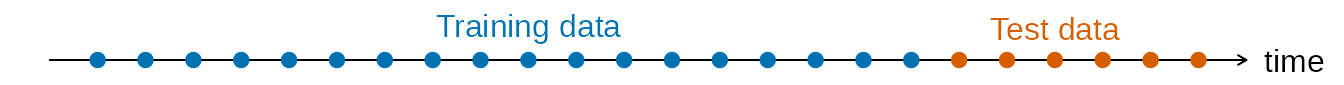
\includegraphics[width=0.95\textwidth]{split.png}

\bigskip
Cross-validation, 1-step ahead:

\smallskip
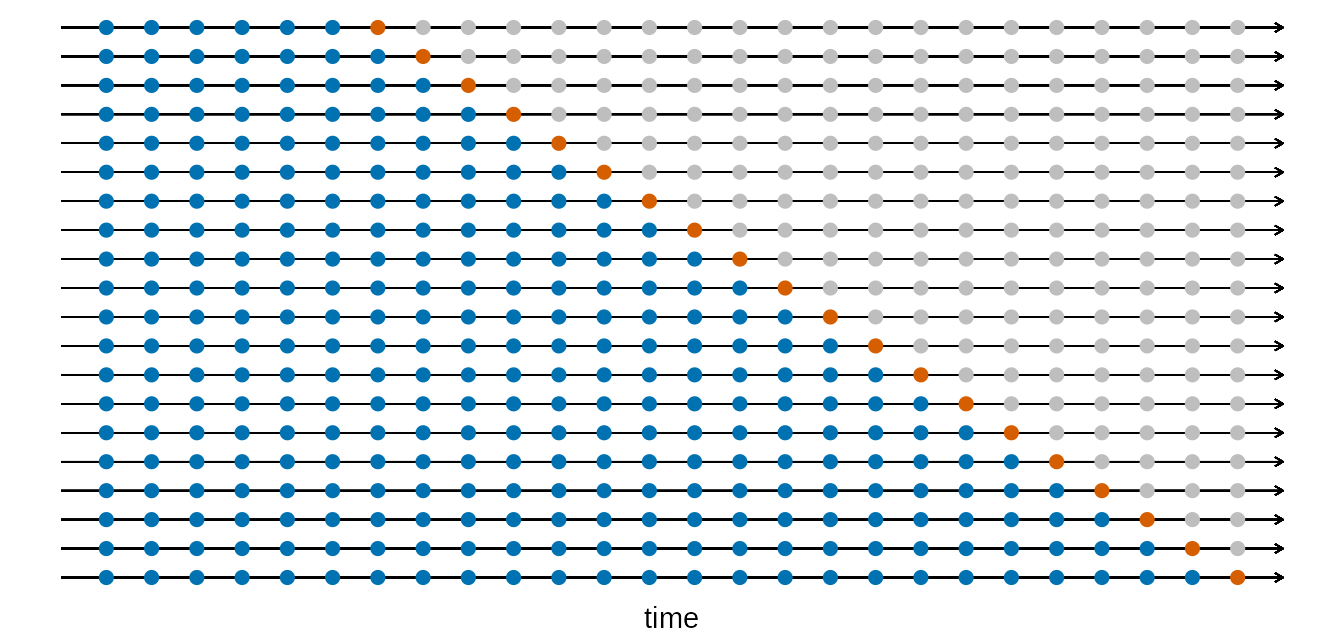
\includegraphics[width=0.95\textwidth]{cv1.png}

\bigskip
Cross-validation, 4-steps ahead: 

\smallskip
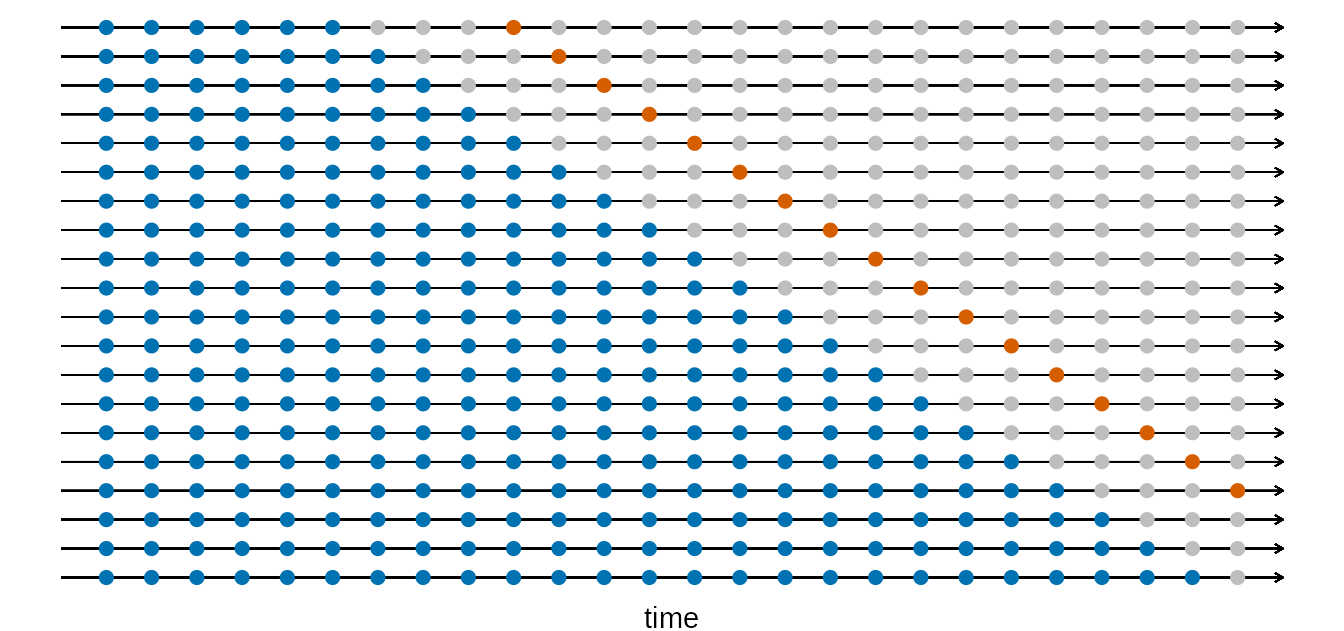
\includegraphics[width=0.95\textwidth]{cv4.png}

\medskip
\caption{Visualization of split-sample and time series cross-validation schemes
  (from HA).} 
\label{fig:split_cv}
\end{figure}

\item Figure \ref{fig:cardio_cv1} then displays the walk-forward predictions
  from time series cross-validation on the cardiovascular mortality
  example. (Recall, these are 4-step ahead forecasts, so the CV scheme is as in
  the bottom panel of Figure \ref{fig:split_cv}.) We can see that the MAE has
  improved a bit from the split-sample forecasts in Figure
  \ref{fig:cardio_split} (from about 9.39 to 8.03). However, the forecasts still
  look biased upwards  

\begin{figure}[htb]
\centering
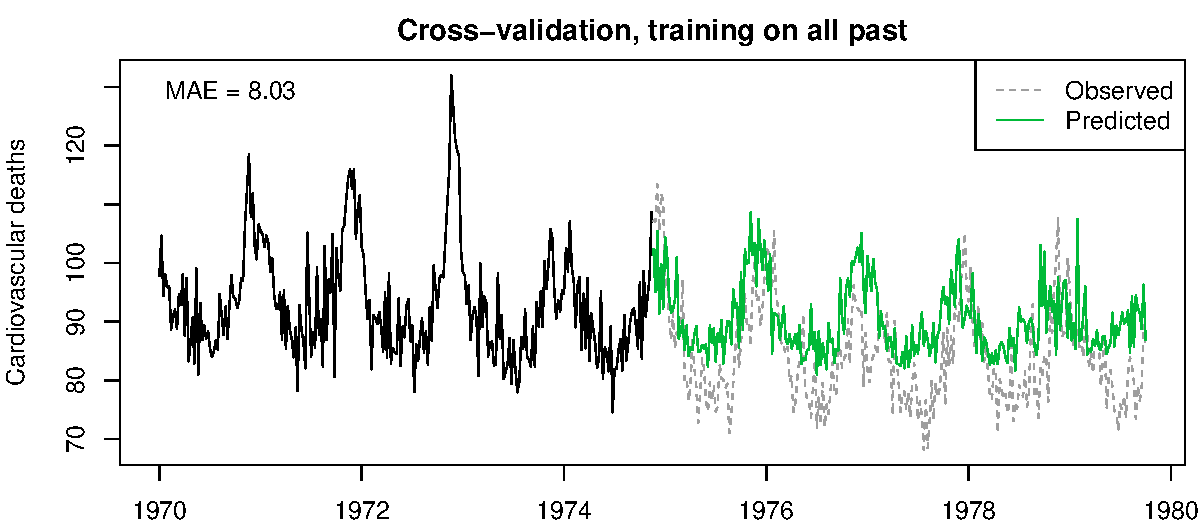
\includegraphics[width=0.9\textwidth]{fig/cardio-cv-1.pdf} 
\caption{Walk-forward forecasts of cardiovascular mortality, made at a 4-week
  ahead horizon, using particulate level as a lagged predictor. The regression
  model is trained on all past.} 
\label{fig:cardio_cv1}

\bigskip
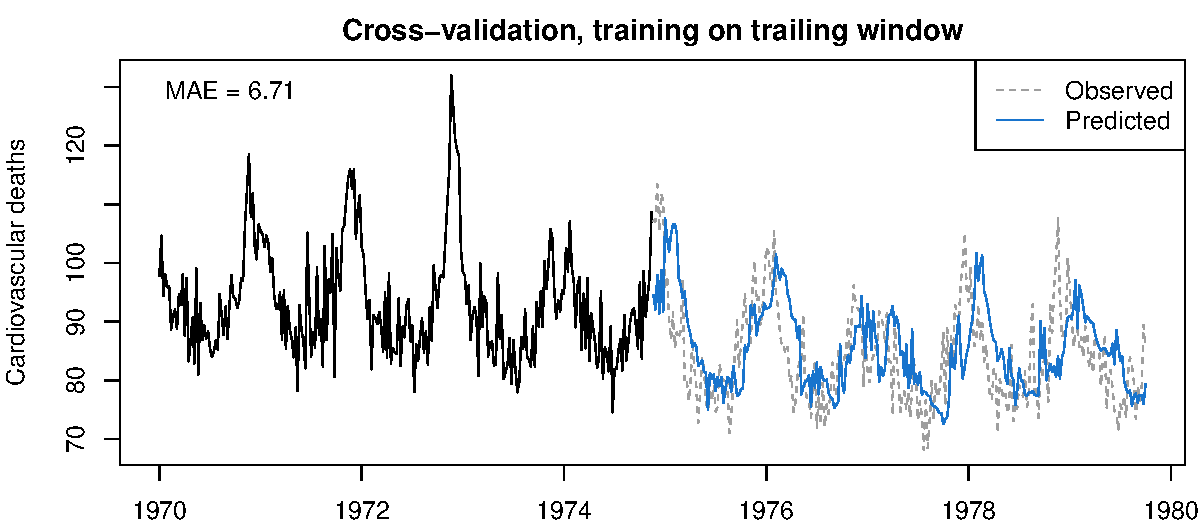
\includegraphics[width=0.9\textwidth]{fig/cardio-cv-2.pdf} 
\caption{As in the above figure, but with the regression model trained on a
  trailing window of 10 weeks.} 
\label{fig:cardio_cv2}
\end{figure}
\end{itemize}

\subsection{Trailing windows}

\begin{itemize}
\item It turns out that we can further improve the forecasts in the
  cardiovascular mortality example by training on a \emph{trailing window},
  rather than on all past. In other words, to fit the regression model we use to 
  make a $k$-step ahead forecast of the response's value at time $t$, instead of 
  solving    
  \[
  \min_{\beta_0,\beta_1} \, \sum_{s=1}^{t-k} (y_s - \beta_0 - \beta_1 x_{s-k})^2
  \]
  we solve
  \[
  \min_{\beta_0,\beta_1} \, \sum_{s={t-k-w+1}}^{t-k} (y_s - \beta_0 - \beta_1
  x_{s-k})^2 
  \]
  for a choice of window length $w$

\item Figure \ref{fig:cardio_cv2} shows such forecasts with a window length $w = 
  10$ (i.e., 10 weeks). We see that it does quite a bit better, both
  qualitatively and in terms of MAE (from about 8.03 to 6.77) 

\item Why does this happen? Because the relationship between cardiovascular
  mortality and particulate level is changing over time. In the language of the
  last lecture, these two series, cardiovascular mortality and particulate
  level, are \emph{not jointly stationary} 

\item Training on a trailing window helps to hone in on the most relevant
  (recent) data for prediction. If the window is too long, then the fitted model
  cannot adapt to nonstationarity as well; if the window is too short, then the
  fitted model may be too volatile (trained on too little data)

\item The choice of window $w$ should be rigorously examined, just like the 
  choice and number of lags. To do so, we can use CV, once again---and to
  reiterate, CV is our main tool to select \emph{tuning parameters} of the
  working model (the number of lags and the length of the trailing window being
  two examples) 
\end{itemize}
\end{document}
